%State the hypotheis of the test. H0 and H1
%State the test.
%State the number from the summation and how the degrees of freedm is calculated. State how the critical value is selected. State how the how test is conducted. State that the resulting data doesn�t allow us to reject H0
%State what rejection would mean. State additional tests are needed to confirm the awesomeness of the chain

\section{Model Validation}

%State that verification of the profile chain via statistical tests is important. State that if P and T are ergodic stochastic sources and can generate similar sequences if they have the same transition probabilities. State that statistical tests can identify if two chains are different at some significant level. 

To assert the closed form profile chain accurately represents the implementation of the algorithm, it must be validated.
Since $T$ and $P$ are ergodic, they can be checked for equivalence using a goodness-of-fit test.
If the goodness-of-fit test indicates the chains are equivalent, they will generate similar sequences and have similar properties when analyzed.
Therefore, generated $P$ chains can be used to analyze the behavior of the algorithm during live execution with changing conditions.

To verify the test chain $T$ is equivalent to the profile chain $P$, a $\chi^2$ goodness-of-fit test is employed.
The null-hypothesis of this test ($H_{0}$) asserts the profile chain $P$ is equivalent to the test chain $T$:

\[ H_{0}: T = P \]

With an alternative hypothesis that the two chains are not equivalent:

\[ H_{1}: T \neq P \]

The $\chi^2$ test measures the goodness-of-fit for a complete chain by combining the measurements of goodness of fit for the transitions away from each state.
Therefore, the goodness of fit test for the chain is a summation of tests for each state:\cite{MARKOV3}

\[ \chi^2 = \sum_{i}^{m} \sum_{j}^{m} = \frac{n_{i}(P_{ij}-T_{ij})^2}{P_{ij}} \]

Where $n_{i}$ is the number of times the state $i$ was observed in the input sequence used to construct the test chain $T$.
The summation is distributed as $\chi^2$ with $m(m-1)$ degrees of freedom if all entries in $P_{ij}$ are non-zero.
In this work, all transitions in the profile Markov chain $P$ are non-zero when $0<p<1.0$.
However, the probability of some transitions may be extremely small.
The $\chi^2$ value was compared to a critical value (CV) giving a measure of how likely it was $H_{0}$ could not be rejected.
This work selected an $\alpha = 0.05$ significance level to accept the hypothesis $T=P$.

If the hypothesis $H_{0}$ were to be rejected, it would indicate the test chain and profile chain differ significantly.
As a consequence of rejecting the hypothesis, the implementation would have behavior from the generated closed form solution.

\begin{figure}
    \centering
    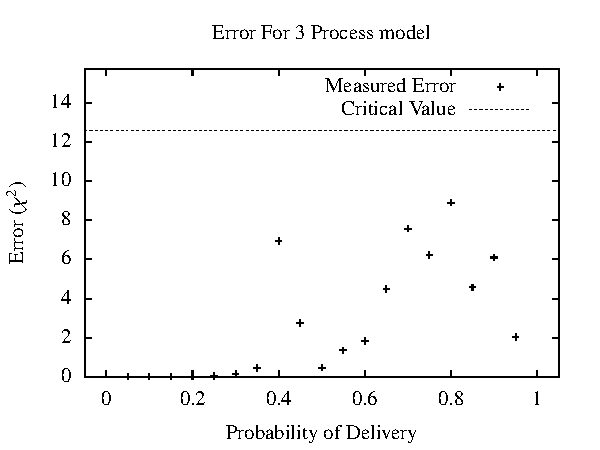
\includegraphics[width=0.65\textwidth]{3process.pdf}
    \caption{Observed error comparing test chains (T) to profile chains (P) with 3 processes.}
    \label{fig:3process}
\end{figure}

\begin{figure}
    \centering
    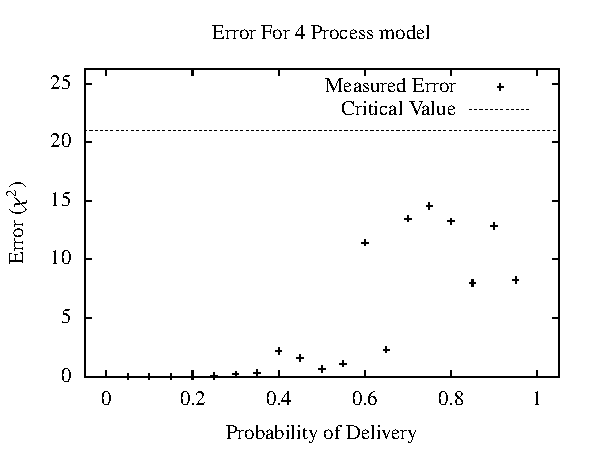
\includegraphics[width=0.65\textwidth]{4process.pdf}
    \caption{Observed error comparing test chains (T) to profile chains (P) with 4 processes.}
    \label{fig:4process}
\end{figure}

\begin{figure}
    \centering
    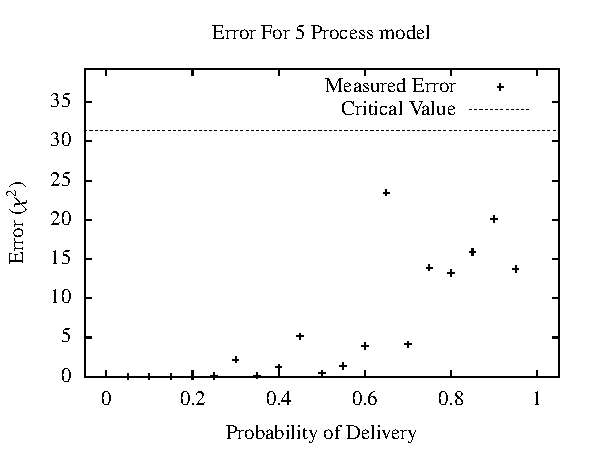
\includegraphics[width=0.65\textwidth]{5process.pdf}
    \caption{Observed error comparing test chains (T) to profile chains (P) with 5 processes.}
    \label{fig:5process}
\end{figure}

\begin{figure}
    \centering
    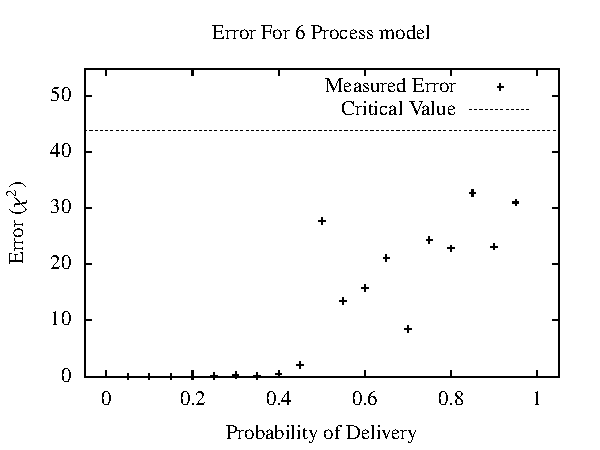
\includegraphics[width=0.65\textwidth]{6process.pdf}
    \caption{Observed error comparing test chains (T) to profile chains (P) with 6 processes.}
    \label{fig:6process}
\end{figure}

Figures \ref{fig:3process}, \ref{fig:4process}, \ref{fig:5process} and \ref{fig:6process} show the observed error for message delivery probabilities between 0.05 and 0.95.
The dotted line in each figure indicates the critical level where $H_{0}$ should be rejected.
Since all of the plotted points are below and not close to the dotted line, we cannot reject $H_{0}$ at the 0.05 significance.
Table \ref{tab:chisummary} shows the p-value for the worst observed error for each number of processes.
This indicates the profile chains ($P$) are representative of the behavior of the algorithm's implementation.

\begin{table}
\centering
\begin{tabular}{ c | c c c c}
  \hline
  Processes & Degrees of Freedom & Worst Error & $\Pr(WorstError)$ & p-value \\ \hline
  3 & 6 & 8.90 & 0.80 & 0.18 \\
  4 & 12 & 14.55 & 0.75 & 0.27 \\
  5 & 20 & 23.47 & 0.65 & 0.27 \\
  6 & 30 & 32.69 & 0.85 & 0.34 \\
\end{tabular}
\caption{Summary of $\chi^2$ tests performed.}
\label{tab:chisummary}
\end{table}

